\chapter{Literature review}
\label{ch:literature_review}

L\'evy search strategies lie at the intersection of ecology, statistical physics, and algorithmic search, because they provide a simple scale-free rule for exploring environments where targets are sparse and sensory information is limited. The influential model of Viswanathan \emph{et al.} suggested that inverse-square L\'evy walks (corresponding to $\alpha \approx 1$) can be near-optimal under minimal assumptions and has since become a standard reference point~\cite{viswanathan1999optimizing}. At the same time, subsequent empirical re-analyses and theoretical work have produced sharp critiques and mutually contradictory conclusions about whether $\alpha \approx 1$ is optimal in two dimensions, and even about what ``optimal'' should mean once objectives and modeling choices are specified~\cite{buldyrev2021comment,edwards2007revisiting,james2011assessing,levernier2020inverse,palyulin2014levy,plank2008optimal}. This lack of consensus motivates a systematic revisit of the classical framework and a careful separation of (i)~the modeling assumptions and (ii)~the performance criteria. Throughout this review, we use \emph{mean first-passage time (MFPT)} to the first detection and \emph{throughput} (long-run encounter rate, targets per unit distance or time) as the two main measures of performance.

This chapter first clarifies the distinction between L\'evy flights and L\'evy walks (Section~\ref{sec:flights_vs_walks}), then recalls the core Viswanathan model and its assumptions (Section~\ref{sec:core_model}), reviews results supporting L\'evy-type optimality under specific conditions (Section~\ref{sec:positive}), followed by critical and negative results that emphasize context dependence (Section~\ref{sec:negative}). Section~\ref{sec:refinements} summarizes refinements and responses that identify parameter regimes where $\alpha \approx 1$ remains strongly advantageous. Finally, Section~\ref{sec:gaps} states the outstanding questions that motivate the benchmark developed in this thesis.

%-----------------------------------------------------------
\section{L\'evy flights versus L\'evy walks}
\label{sec:flights_vs_walks}

Before reviewing the foraging literature it is important to distinguish two related but physically different stochastic models that are frequently conflated in the literature.

A \textbf{L\'evy flight} is a random walk in which the displacement at each discrete step is drawn from a heavy-tailed (power-law) distribution, and each step is completed \emph{instantaneously}---that is, every step occupies the same unit of time regardless of its length~\cite{shlesinger1986walks}. In continuous time, this means that a single step of length~$\ell$ is traversed in one time unit, implying an effective speed proportional to~$\ell$. As a consequence, L\'evy flights can produce arbitrarily large instantaneous velocities, and the mean-square displacement may diverge: the process is superdiffusive but unphysical when a finite speed is required.

A \textbf{L\'evy walk}, by contrast, is a coupled continuous-time random walk in which the walker moves at \emph{constant speed}~$v$~\cite{shlesinger1986walks,zaburdaev2015levy}. A step of length~$\ell$ takes a time $\tau = \ell/v$, so long relocations are correspondingly time-consuming. The resulting mean-square displacement is finite at any finite time (though it can still grow faster than diffusion), and the velocity is bounded. L\'evy walks are therefore the physically appropriate model for organisms or robots moving through space, which is why the foraging literature overwhelmingly studies constant-speed motion~\cite{viswanathan1999optimizing,bartumeus2005animal}.

\begin{figure}[htb]
\centering
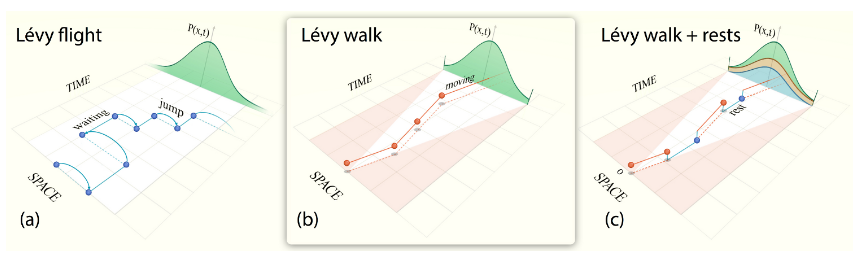
\includegraphics[width=0.85\textwidth]{images/levy_walks.png}
\caption{Schematic comparison of (a)~a L\'evy flight, in which each step is completed instantaneously (``jump''), (b)~a L\'evy walk, in which the walker moves at constant speed between turning points, and (c)~a L\'evy walk with rests, where the walker pauses at each turning point before resuming.  The upper curves show the propagator $P(x,t)$ at a fixed time.  Adapted from Zaburdaev et~al.~\cite{zaburdaev2015levy}.}
\label{fig:levy_walks}
\end{figure}

Despite this clear conceptual distinction, many publications in the foraging literature use the term ``L\'evy flight'' when the underlying model is in fact a constant-speed walk~\cite{viswanathan1999optimizing,bartumeus2002optimizing,edwards2007revisiting}. The confusion was noted already by Shlesinger and Klafter in the original chapter that introduced the terminology~\cite{shlesinger1986walks}, and persists in recent work. In this thesis, the simulation is a L\'evy \emph{walk}: the searcher moves at constant unit speed and each flight of length~$\ell$ takes time~$\ell$. Where we use the phrase ``L\'evy flight'' (following common usage in the foraging community), it should be understood as referring to this constant-speed process, not to instantaneous jumps.

%-----------------------------------------------------------
\section{Core foraging model and assumptions}
\label{sec:core_model}
The L\'evy foraging hypothesis was formalized by Viswanathan \emph{et al.} in a minimal random search model in $d=1,2$ with homogeneous target fields, constant speed, finite detection radius $r_v$, and no memory beyond immediate detection~\cite{viswanathan1999optimizing}. The model builds on earlier ideas from fractals and anomalous transport~\cite{mandelbrot1967coast,shlesinger1986walks,shlesinger1993strange} and on early empirical reports of scale-free movement patterns~\cite{cole1995fractal,focardi1996ungulates,heinrich1979resource,viswanathan1996albatross}. Step lengths are drawn from a power law
\[
P(\ell) \propto \ell^{-\mu},\quad \mu>1,
\]
which corresponds to a L\'evy-stable index $\alpha=\mu-1$.

The Viswanathan model specifies a searcher that executes a sequence of straight-line flights in uniformly random directions. When the searcher passes within a detection radius~$r_v$ of a target, it registers a detection. Two interaction modes are considered: \emph{destructive} search (each target is removed upon detection) and \emph{nondestructive} search (targets persist and may be revisited). In the destructive setting, Viswanathan \emph{et al.} derived an asymptotic expression for the mean number of flights~$N$ required per detection, $N \sim (\lambda/r_v)^{(\mu-1)/2}$, where $\lambda = 1/(2\rho r_v)$ is the mean free path~\cite{viswanathan1999optimizing}. The throughput objective is $\eta = 1/(N\langle\ell\rangle)$, where $\langle\ell\rangle$ is the mean flight length. Under their idealized assumptions (sparse targets in an effectively infinite homogeneous domain, no drift, and a particular treatment of revisits), both the destructive and the nondestructive cases in 2D exhibit an interior optimum at $\mu \simeq 2$ (equivalently $\alpha \simeq 1$). The nondestructive advantage is more pronounced because revisits additionally penalize short-range (Brownian-like) strategies that remain in the neighborhood of already-detected targets~\cite{viswanathan1999optimizing}. Numerical experiments on periodic domains confirmed these asymptotic predictions~\cite{viswanathan1999optimizing}.

Viswanathan \emph{et al.} also fitted heavy-tailed or exponential models to GPS movement data for albatrosses, deer, and bumblebees and reported $\mu \approx 2$ in large open environments, with more exponential-like behavior in confined settings~\cite{focardi1996ungulates,heinrich1979resource,viswanathan1996albatross,viswanathan1999optimizing}. This empirical component attracted widespread attention, although later re-analyses argued that such fits are statistically fragile and sensitive to data processing choices (see Section~\ref{sec:negative})~\cite{edwards2007revisiting,james2011assessing,plank2008optimal}.

\begin{figure}[htb]
\centering
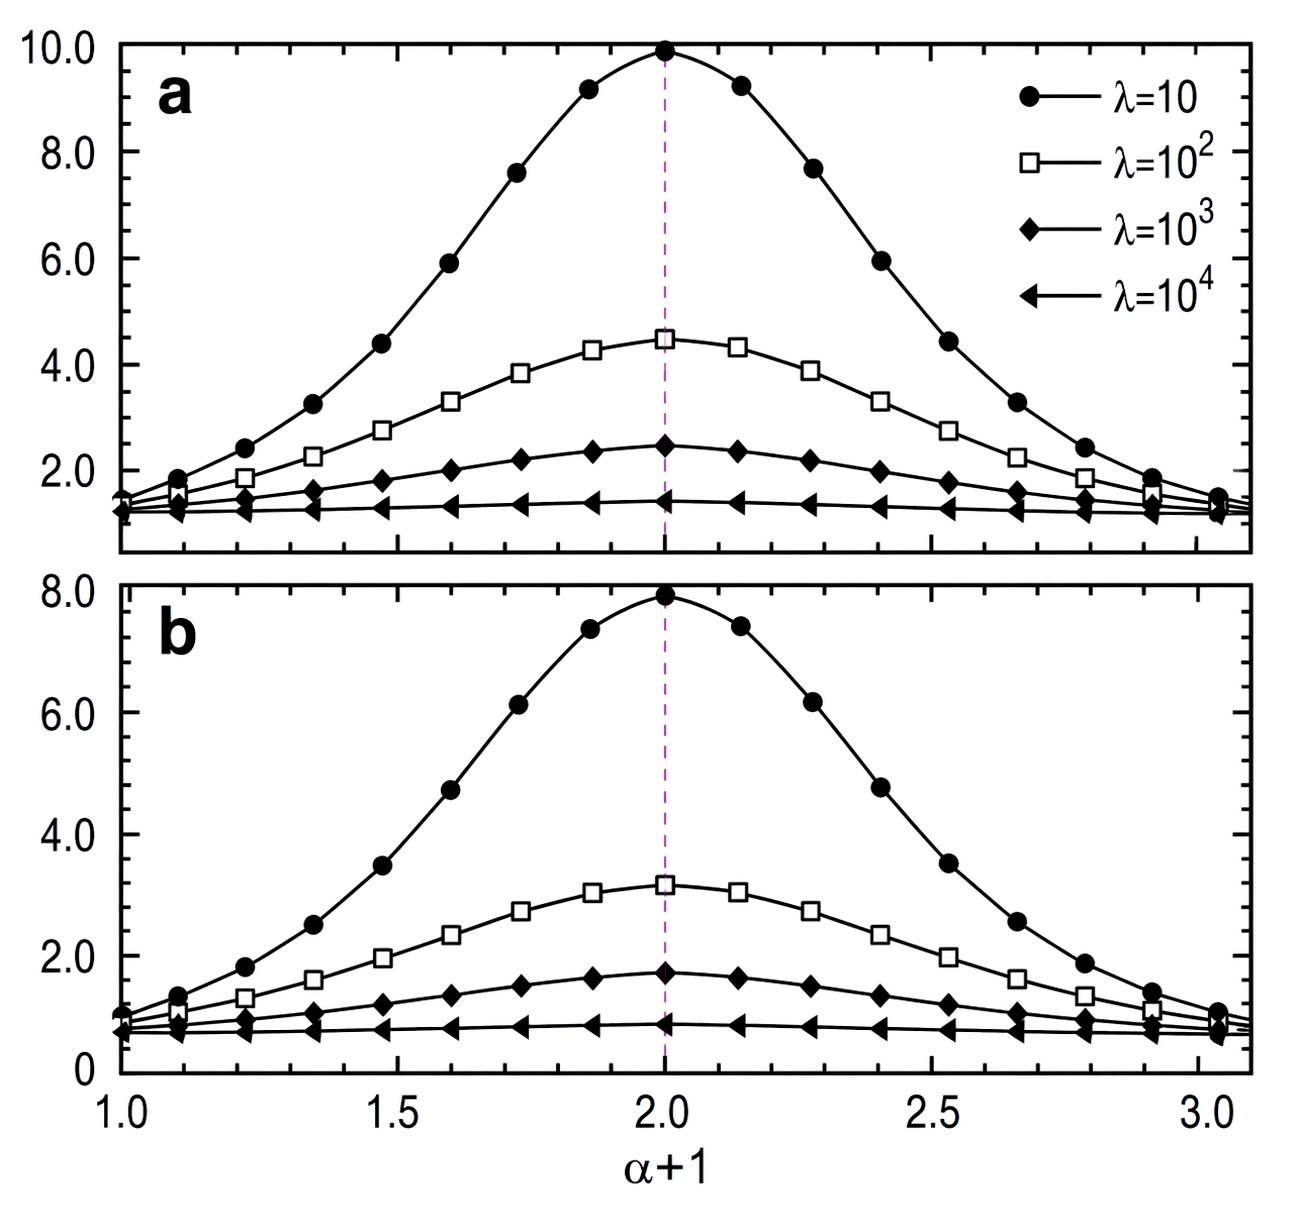
\includegraphics[width=0.5\linewidth]{images/viswanathan1999.png}
\caption{The product of the mean free path~$\lambda$ and the foraging efficiency~$\eta$ plotted against the L\'evy parameter $\alpha+1$ (reproduced from the original Viswanathan~et~al.\ (1999) paper~\cite{viswanathan1999optimizing}). The peak at $\mu \approx 2$ in the nondestructive case is the central prediction of the L\'evy foraging hypothesis.}
\label{fig:viswanathan_original}
\end{figure}

The classical framework therefore implicitly fixes several design choices: (i)~dimension~$d$; (ii)~destructive vs.\ nondestructive interactions; (iii)~boundary conditions and finite-size effects; (iv)~the performance objective (throughput vs.\ MFPT); and (v)~the specific mechanism by which nondestructive revisits are handled (e.g., renewal time, jump-off distance, or immediate restart). Much of the later literature can be read as asking what happens when one (or several) of these assumptions is changed.

%-----------------------------------------------------------
\section{Evidence in favor of L\'evy-type optimality}
\label{sec:positive}
A substantial body of work supports the claim that L\'evy-like dynamics can be efficient search strategies under clearly stated conditions. We organize these results by the type of evidence: theoretical and numerical analyses in controlled models, empirical fits to animal movement data, and evolutionary arguments.

\paragraph{Theoretical and numerical analyses.}
Bartumeus \emph{et al.}~\cite{bartumeus2002optimizing} compared L\'evy and Brownian walkers searching for randomly placed targets in continuous 1D and 2D domains. Using throughput-based performance metrics, they demonstrated that heavy-tailed relocations reduce the probability of local oversampling (repeatedly scanning already-cleared areas) and improve encounter rates for sparse targets. Their numerical simulations showed optimal exponents near $\mu \simeq 2$ in 2D, consistent with the Viswanathan prediction, and importantly highlighted that the advantage arises from the balance between local exploration (short flights) and long-range relocation (occasional ballistic segments). Raposo \emph{et al.}~\cite{raposo2003dynamical} extended this analysis to probe the dynamical robustness of the L\'evy advantage. They showed that the efficiency peak near $\mu = 2$ is not an artifact of a single parameter choice but persists under moderate perturbations of the target density and domain size. However, they also noted that the peak broadens and flattens as the environment becomes denser, foreshadowing the density dependence studied in detail in this thesis.

For revisitable targets, Santos \emph{et al.}~\cite{santos2004optimal} introduced explicit nondestructive mechanics through a renewal time~$\tau$ and a restart distance~$l_c$ in effectively unbounded 1D settings. Their key result is a two-parameter phase diagram: the preferred exponent drifts toward $\mu \to 2$ as renewal becomes fast ($\tau \to 0$) and restart distances become small ($l_c \to 0$), and toward $\mu \to 1$ (ballistic) as renewal becomes slow ($\tau \gg 1$). Intermediate regimes exhibit smooth crossovers, indicating that ``$\alpha \approx 1$ optimality'' corresponds to a specific corner of a larger parameter space rather than a universal law.

A different but closely related line of work studies \emph{intermittent search}, where the searcher alternates between a slow detection phase and a fast relocation phase without detection. B{\'e}nichou \emph{et al.}~\cite{benichou2006twodimensional} derived MFPT-optimal switching rules for intermittent searchers in 2D confined domains and showed that long relocations can substantially reduce MFPT in sparse regimes. Their comprehensive review~\cite{benichou2011intermittent} synthesizes these results across dimensions and geometries, clarifying that the advantage of intermittent strategies over purely diffusive exploration is largest when the ratio of domain size to detection radius is large---analogous to the sparse-target condition in the foraging literature. Lomholt \emph{et al.}~\cite{lomholt2008levy} further argued that L\'evy-like relocations can be advantageous within intermittent processes, provided the relocation phase duration is drawn from a heavy-tailed distribution. They showed that in certain regimes the MFPT scales as $T \sim L^{d_w}$ with a walk dimension $d_w < 2$, outperforming both ballistic and Brownian intermittent strategies.

Several extensions examine modifications of L\'evy motion itself. Chen \emph{et al.}~\cite{chen2018tempered} studied \emph{tempered L\'evy flights}, in which the power-law tail is exponentially damped beyond a characteristic scale. They showed that an optimal tempering level exists for MFPT-based search, interpolating between heavy-tailed motion (efficient exploration of distant regions) and effectively short-tailed motion (efficient local scanning). The optimal tempering scale is related to the typical inter-target distance, providing a connection to the truncation parameters ($l_{\min}$, $l_{\max}$) studied in this thesis. Padash \emph{et al.}~\cite{padash2022asymmetric} analyzed asymmetric (skewed) L\'evy flights and reported that controlled asymmetry can reduce MFPT compared to symmetric L\'evy and Brownian cases in 1D settings, suggesting that directional bias can complement the advantages of heavy-tailed relocation.

\paragraph{Empirical evidence.}
On the empirical side, Humphries \emph{et al.}~\cite{humphries2012foraging} analyzed high-resolution tracking data from 55 marine predators (including sharks, tuna, and ocean sunfish) using rigorous maximum-likelihood model selection. They reported that truncated power-law models outperformed exponential alternatives for the majority of individuals, with inferred exponents clustering near $\mu \approx 2$ during search phases in open water but shifting toward exponential behavior during area-restricted search near prey patches. Garg and Kello~\cite{garg2021efficient} documented similar L\'evy-like patterns in virtual human foraging experiments, where participants searching for hidden targets in featureless environments spontaneously adopted heavy-tailed movement strategies. Reynolds \emph{et al.}~\cite{reynolds2018rural} extended these findings to rural human foragers (Juchit\'an de Zaragoza, Mexico), reporting truncated power-law step-length distributions with $\mu \approx 2$ during mushroom and firewood collection in low-density environments. However, the inferred exponents depend on segmentation methods and the candidate model class, so these empirical results should be interpreted with appropriate caveats (see Section~\ref{sec:negative}).

\paragraph{Evolutionary arguments.}
Wosniack \emph{et al.}~\cite{wosniack2017evolutionary} used evolutionary simulations in which foraging efficiency (throughput) determined reproductive fitness. Starting from random initial exponents, populations evolving under sparse-resource conditions on periodic domains repeatedly converged to heavy-tailed exponents near $\mu \approx 2$, suggesting that L\'evy-like motion can be an evolutionarily stable strategy under a Viswanathan-style set of assumptions. The evolutionary stability lends additional theoretical support but also inherits the same model dependence: the selected exponent depends on the fitness function, boundary conditions, and target dynamics.

\paragraph{Summary.}
Under their stated assumptions (typically homogeneous domains, weak or no bias, sparse targets, and a fixed objective such as MFPT or throughput), these works collectively demonstrate that L\'evy-type strategies can outperform Brownian motion in low-information search. The advantage is most robust when targets are sparse, the searcher has no memory or cues, and the performance objective penalizes local oversampling. This motivates the central questions of this thesis (Section~\ref{sec:research_questions}): when does an interior optimum near $\alpha \approx 1$ exist in 2D, and how sensitive is it to sparsity and scale parameters?

%-----------------------------------------------------------
\section{Negative and contradictory results}
\label{sec:negative}
In contrast, several influential works question the universality of L\'evy optimality and emphasize strong context dependence. These critiques fall into three categories: empirical re-analyses, theoretical counter-examples in modified environments, and fundamental scaling arguments.

\paragraph{Empirical re-analyses.}
The most influential empirical critique came from Edwards \emph{et al.}~\cite{edwards2007revisiting}, who re-analyzed the same albatross, bee, and deer tracking datasets that had been used to support the L\'evy foraging hypothesis. Using higher-resolution data and rigorous likelihood-based model selection (Akaike information criterion and log-likelihood ratio tests), they showed that exponential-tailed alternatives (including composite Brownian models with two characteristic scales) can outperform pure power-law fits for the albatross and deer data. Critically, they demonstrated that pooling movement data across individuals---a practice common in early L\'evy analyses---can produce spurious apparent scaling: if different individuals move with different characteristic speeds, the pooled step-length distribution can mimic a power law even when each individual's distribution is exponential. This methodological critique prompted the development of more rigorous statistical frameworks. Plank and James~\cite{plank2008optimal} formalized a likelihood-based testing framework specifically designed to distinguish L\'evy walks from composite Brownian models, accounting for truncation effects and finite sample sizes. James \emph{et al.}~\cite{james2011assessing} extended this approach and applied it to multiple empirical datasets, often finding that composite Brownian or truncated exponential models provided better fits than L\'evy models. These results do not rule out heavy tails, but they substantially weaken the claim that empirical movement data robustly supports exact L\'evy laws, and they highlight the importance of per-individual analysis and proper model selection.

\paragraph{Theoretical counter-examples.}
Palyulin \emph{et al.}~\cite{palyulin2014levy} considered environments with drift (external flows or biased motion) and showed that L\'evy flights do not necessarily minimize MFPT once bias is present. In a 1D absorbing-boundary problem with constant drift, they found that for weak drift, L\'evy flights with $\alpha < 2$ can still outperform Brownian motion, but as the drift strength increases, a crossover occurs: Brownian motion becomes optimal for intermediate drift, and ballistic motion becomes optimal for strong drift. In 2D, the interaction between drift direction and the isotropic L\'evy relocation produces even more complex behavior, and the optimal strategy depends on the relative magnitudes of drift, detection radius, and inter-target distance. Volpe and Volpe~\cite{volpe2017topography} studied active particles in structured 2D landscapes with varying topography (rugged potential energy surfaces). They demonstrated that environmental heterogeneity can shift the MFPT-optimal strategy toward more local, Brownian-like exploration, because long ballistic flights in rugged landscapes are frequently interrupted by barriers, negating the advantage of superdiffusive exploration.

\paragraph{Fundamental scaling critique.}
A direct theoretical challenge to ``universal $\alpha \approx 1$ optimality in 2D'' was given by Levernier \emph{et al.}~\cite{levernier2020inverse} for destructive search in $d\ge2$. Using a first-passage approach, they derived asymptotic encounter-rate scaling and showed that, in $d\ge2$, the throughput scales linearly with target density $\rho$ for \emph{all} $\alpha\in(0,2)$: $\eta \sim C(\alpha)\,\rho$ as $\rho \to 0$. This means that changing~$\alpha$ affects only the prefactor~$C(\alpha)$, not the functional dependence on~$\rho$, so there is no parametrically superior scaling as targets become sparse. Furthermore, they showed that the prefactor~$C(\alpha)$ depends sensitively on microscopic implementation choices (cutoff scales, restart distances, detection geometry), and different choices can shift the best-performing~$\alpha$ anywhere across $(0,2)$, undermining any claim to a universal optimum in $d\ge2$. This stands in contrast to the 1D case, where the scaling exponent itself depends on~$\alpha$ and produces a genuine scaling advantage.

\paragraph{Recent critique: model artefact argument.}
Most recently, Pyke \emph{et al.}~\cite{pyke2026artefact} argued that the L\'evy foraging hypothesis is a ``model artefact.'' Through computer simulations of the standard Viswanathan model, they identified two artefactual processes that both intensify as~$\mu$ increases from~1 to~3: (i)~an increase in quick immediate revisits to food locations that happen to be near one another (revisits occurring after few intervening steps with no intervening visits to other targets), and (ii)~an increase in path resurveying (the walker repeatedly scanning previously explored territory). Pyke \emph{et al.} argued that these two processes are responsible for the decline in efficiency at $\mu > 2$, and that slight modeling modifications---such as preventing immediate revisits or penalizing path overlap---can eliminate or shift the efficiency peak, thereby removing the apparent optimality at $\mu = 2$. This critique reinforces the call to interpret L\'evy optimality as contingent on specific model rules rather than as a robust property of random search.

\paragraph{Summary.}
Overall, these results challenge three pillars of the classical hypothesis: robustness of empirical power-law fits~\cite{edwards2007revisiting,james2011assessing,plank2008optimal}, optimality in biased or structured environments~\cite{palyulin2014levy,volpe2017topography}, and universality of an $\alpha\simeq 1$ optimum in 2D~\cite{levernier2020inverse,pyke2026artefact}. Importantly, critical studies typically focus on a single objective (often MFPT or a related asymptotic scaling) and rarely compare MFPT and long-run throughput side by side under identical assumptions. This motivates a unified framework that can systematically vary assumptions and evaluate both objectives.

%-----------------------------------------------------------
\section{Refinements and responses}
\label{sec:refinements}
Several works attempt to reconcile supportive and critical results by identifying regimes where L\'evy-type strategies remain sharply advantageous.

Buldyrev \emph{et al.}~\cite{buldyrev2021comment} responded directly to the Levernier \emph{et al.} critique~\cite{levernier2020inverse} by focusing on a nondestructive ``hide-and-seek'' limit in 2D, where targets are immediately revisitable and the restart distance is close to the detection radius. Introducing the parameter $\delta = l_c/r_v - 1$ and analyzing the limit $\delta \to 0$, they showed that the encounter rate develops a sharp maximum at $\alpha=1$ ($\mu = 2$), with the relative gain of the optimal exponent over other exponents growing as~$\delta$ decreases. Specifically, the ratio $\eta(\alpha=1)/\eta(\alpha=0.5)$ increases from approximately~1.05 at $\delta = 1$ to over~1.5 at $\delta = 0.01$, demonstrating that the ``model-dependent prefactor'' identified by Levernier \emph{et al.} can be substantial in physically relevant regimes. At the same time, their analysis also highlights that this is a singular regime: for fixed $\delta>0$ the optimum can flatten and become sensitive to microscopic details (grid resolution, boundary effects, the precise detection mechanism), consistent with the broader message of model dependence.

The Bartumeus \emph{et al.}~\cite{bartumeus2005animal} review provided an important synthesis by identifying the ecological conditions under which L\'evy-type search is expected to be advantageous. They argued that L\'evy optimality requires three conditions to hold simultaneously: (1)~targets must be sparse relative to the detection radius, (2)~the searcher must have no information about target locations beyond immediate detection, and (3)~the environment must be spatially homogeneous at the scale of individual flights. When any of these conditions is violated---for example, if the forager can remember previously visited locations, or if targets are clustered---the L\'evy advantage diminishes or disappears. This framework provides a principled way to understand why different studies reach different conclusions: the disagreements reflect genuinely different parameter regimes rather than methodological errors.

A complementary direction replaces fixed power-law rules with \emph{learned} strategies. Mu{\~n}oz-Gil \emph{et al.}~\cite{munozgil2023optimal} trained reinforcement-learning agents on sparse-target environments matching the Viswanathan setup and showed that the learned policies can match or slightly exceed the efficiency of the best L\'evy exponent, achieving efficiency gains of 5--15\% over the optimal power-law walker. Kaur \emph{et al.}~\cite{kaur2023adaptive} and Caraglio \emph{et al.}~\cite{caraglio2024learning} extended this approach to active Brownian particles with intermittent strategies, showing that learned switching policies outperform fixed L\'evy exponents, particularly in heterogeneous environments. These results suggest that power-law motion, while near-optimal within its parametric family, is not globally optimal: adaptive strategies that incorporate even rudimentary memory or state information can do better. This motivates a direct comparison between optimized L\'evy flights and adaptive agents (see Chapter~\ref{ch:discussion}, Future work).

%-----------------------------------------------------------
\section{Outstanding questions and motivation for the present study}
\label{sec:gaps}
Across the analytical and empirical work reviewed in Sections~\ref{sec:positive}--\ref{sec:refinements}, the following picture emerges:
\begin{enumerate}
    \item Under idealized assumptions (typically homogeneous domains, weak bias, and carefully specified nondestructive mechanics), Lévy-type motion can maximize throughput or minimize MFPT, and in special limits $\alpha \simeq 1$ becomes sharply optimal~\cite{buldyrev2021comment,raposo2003dynamical,santos2004optimal,viswanathan1999optimizing}.
    \item Once more realistic features are included—finite domains, drift, heterogeneous landscapes, explicit renewal rules, or statistical constraints on empirical fits—the advantage can shrink to constant factors, the best exponent loses universality, and Brownian or ballistic strategies can become preferable in parts of parameter space~\cite{edwards2007revisiting,james2011assessing,levernier2020inverse,palyulin2014levy,plank2008optimal,volpe2017topography}.
\end{enumerate}

What is still missing is a minimal, fully specified 2D computational benchmark in which (a) destructive and nondestructive cases and post-hit departure rules are explicit parameters; (b) MFPT and throughput are both measured under identical settings; and (c) uncertainty is assessed (variance, convergence envelopes) so that claims about the shape and location of an optimum in $\alpha$ are reproducible. The present thesis constructs such a benchmark and uses it to map how the optimal $\alpha$ depends on objectives, interaction rules, and scale parameters, rather than treating Lévy optimality as a universal property of 2D search.
